\part{Methods and implementation}
\label{pa:methods}

\chapter{Ranklust}
\section{Workflow and usage}
The way researchers will work with Ranklust is pretty simple. Step 1 and 2 will
only be required the first time the researcher want to use this app to solve
his/her problem. The rest has to be done every time, unless a previous session
of Cytoscape is loaded with more developed results.

\begin{enumerate}
    \item Install Cytoscape
    \item Install clusterMaker2 plugin through Cytoscape App manager
    \item Upload the network to be clustered and ranked into Cytoscape
    \item Use clusterMaker2 to cluster the network
    \item Use the Ranklust-part of clusterMaker2 to rank the clusters
        \begin{enumerate}
            \item Decide what to score the clusters on
        \end{enumerate}
    \item Use the Ranklust-part of clusterMaker2 to visualize the rankings
\end{enumerate}

Step 6 should show the researchers the ranking of clusters based on what
attributes they wanted to include in step 5a. This ranking represents cluster
biomarkers. The score of the clusters and the order they are ranked in will
decide the state of the patient. State of the patient can be many different
things and what the rankings will mean to the researcher is not yet final. It
will be a new indicator, a biomarker, and information about what it means has to
be gathered empirically through clinical research.

\section{Workflow image examples}
\begin{figure}[h]
    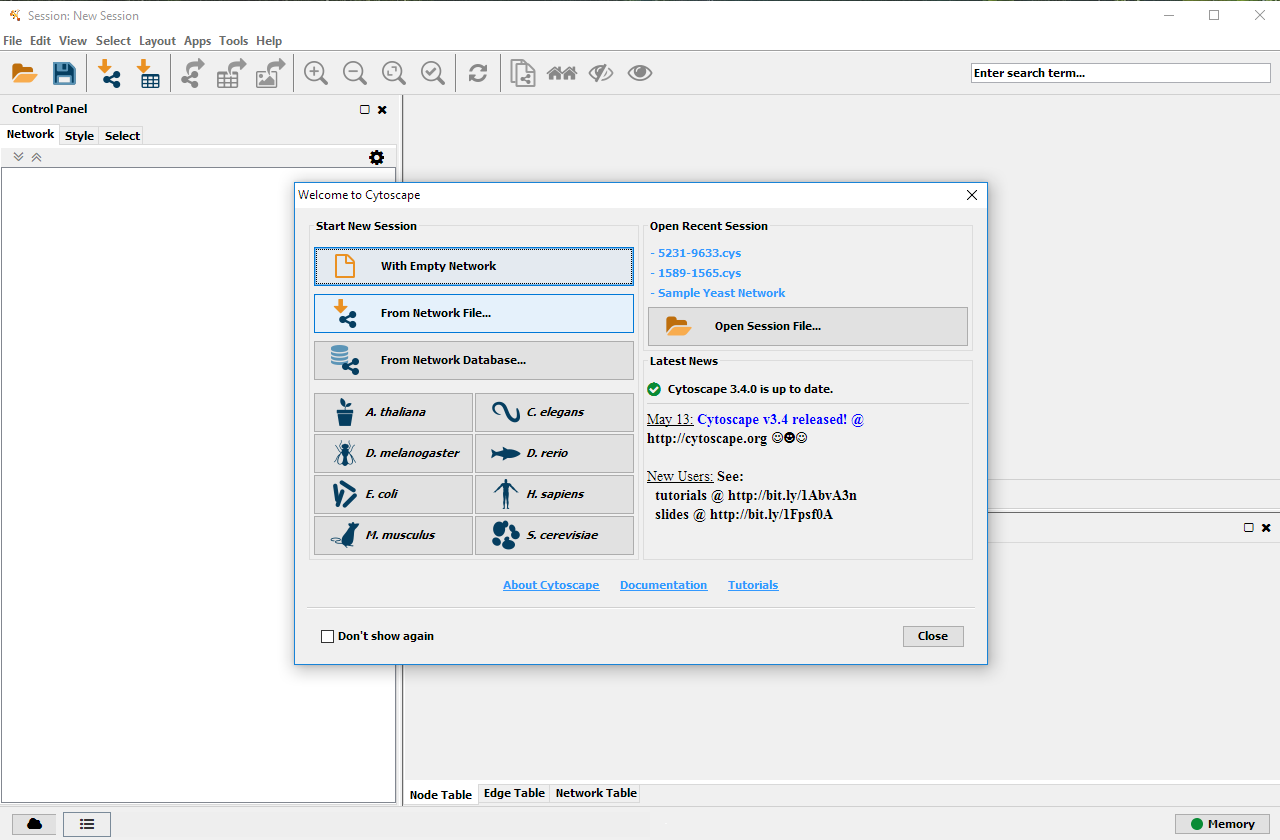
\includegraphics[width=15cm]{1-startup}
\end{figure}
\begin{figure}[h]
    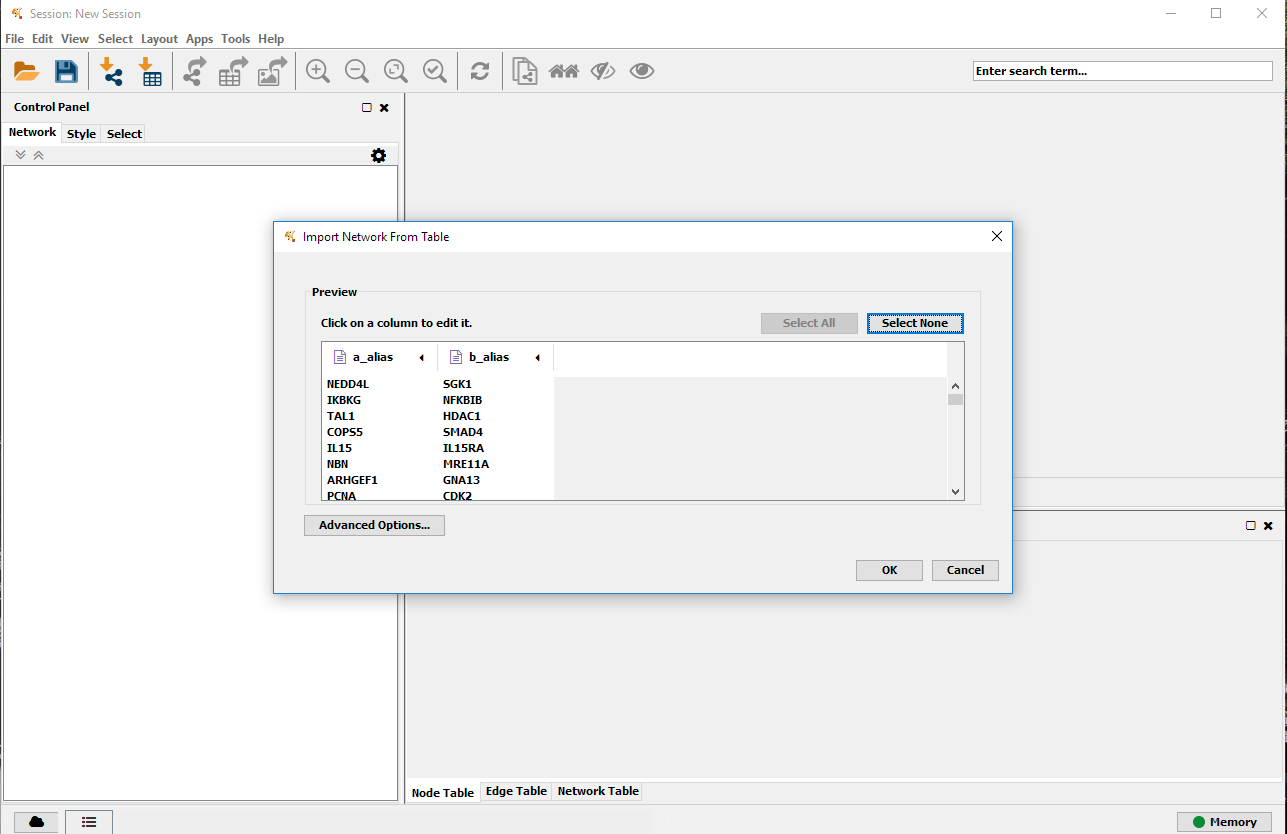
\includegraphics[width=15cm]{2-import}
\end{figure}
\begin{figure}[h]
    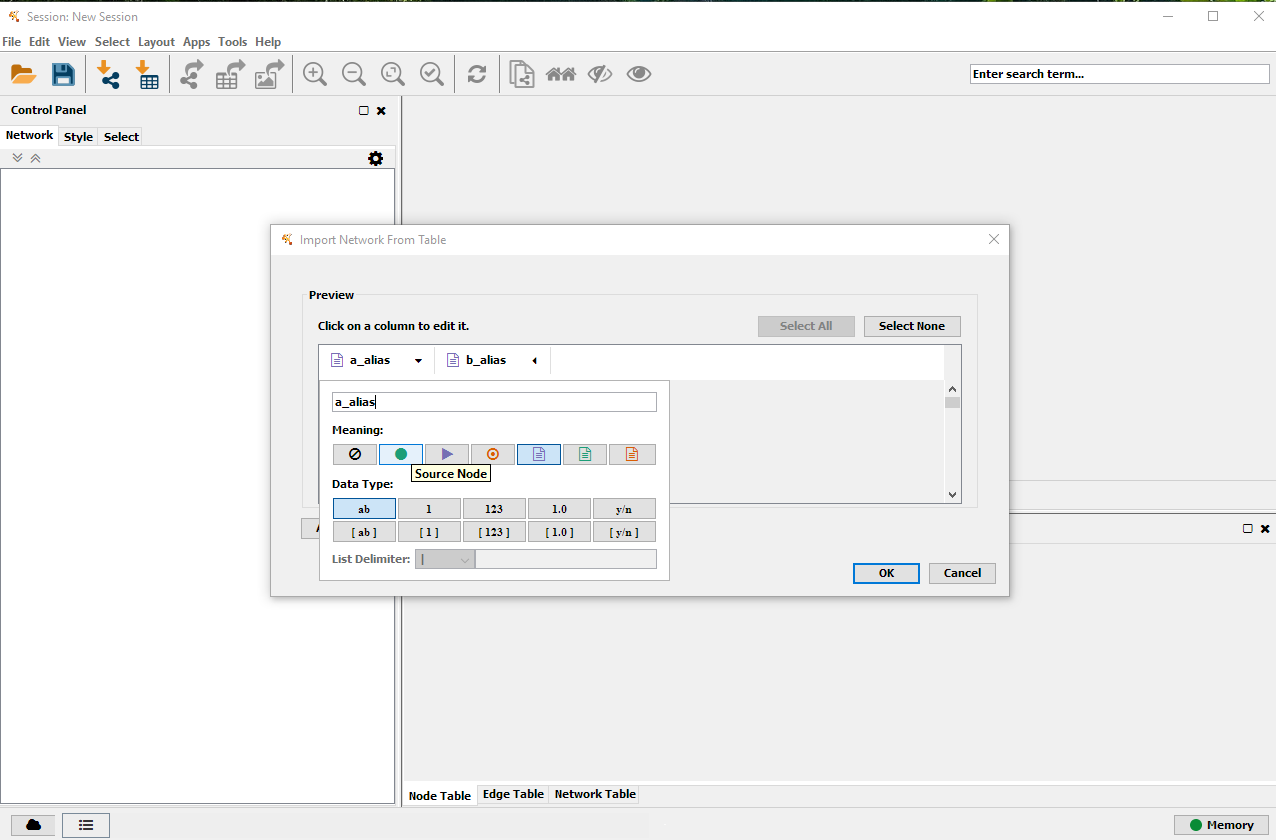
\includegraphics[width=15cm]{3-nodes}
\end{figure}
\begin{figure}[h]
    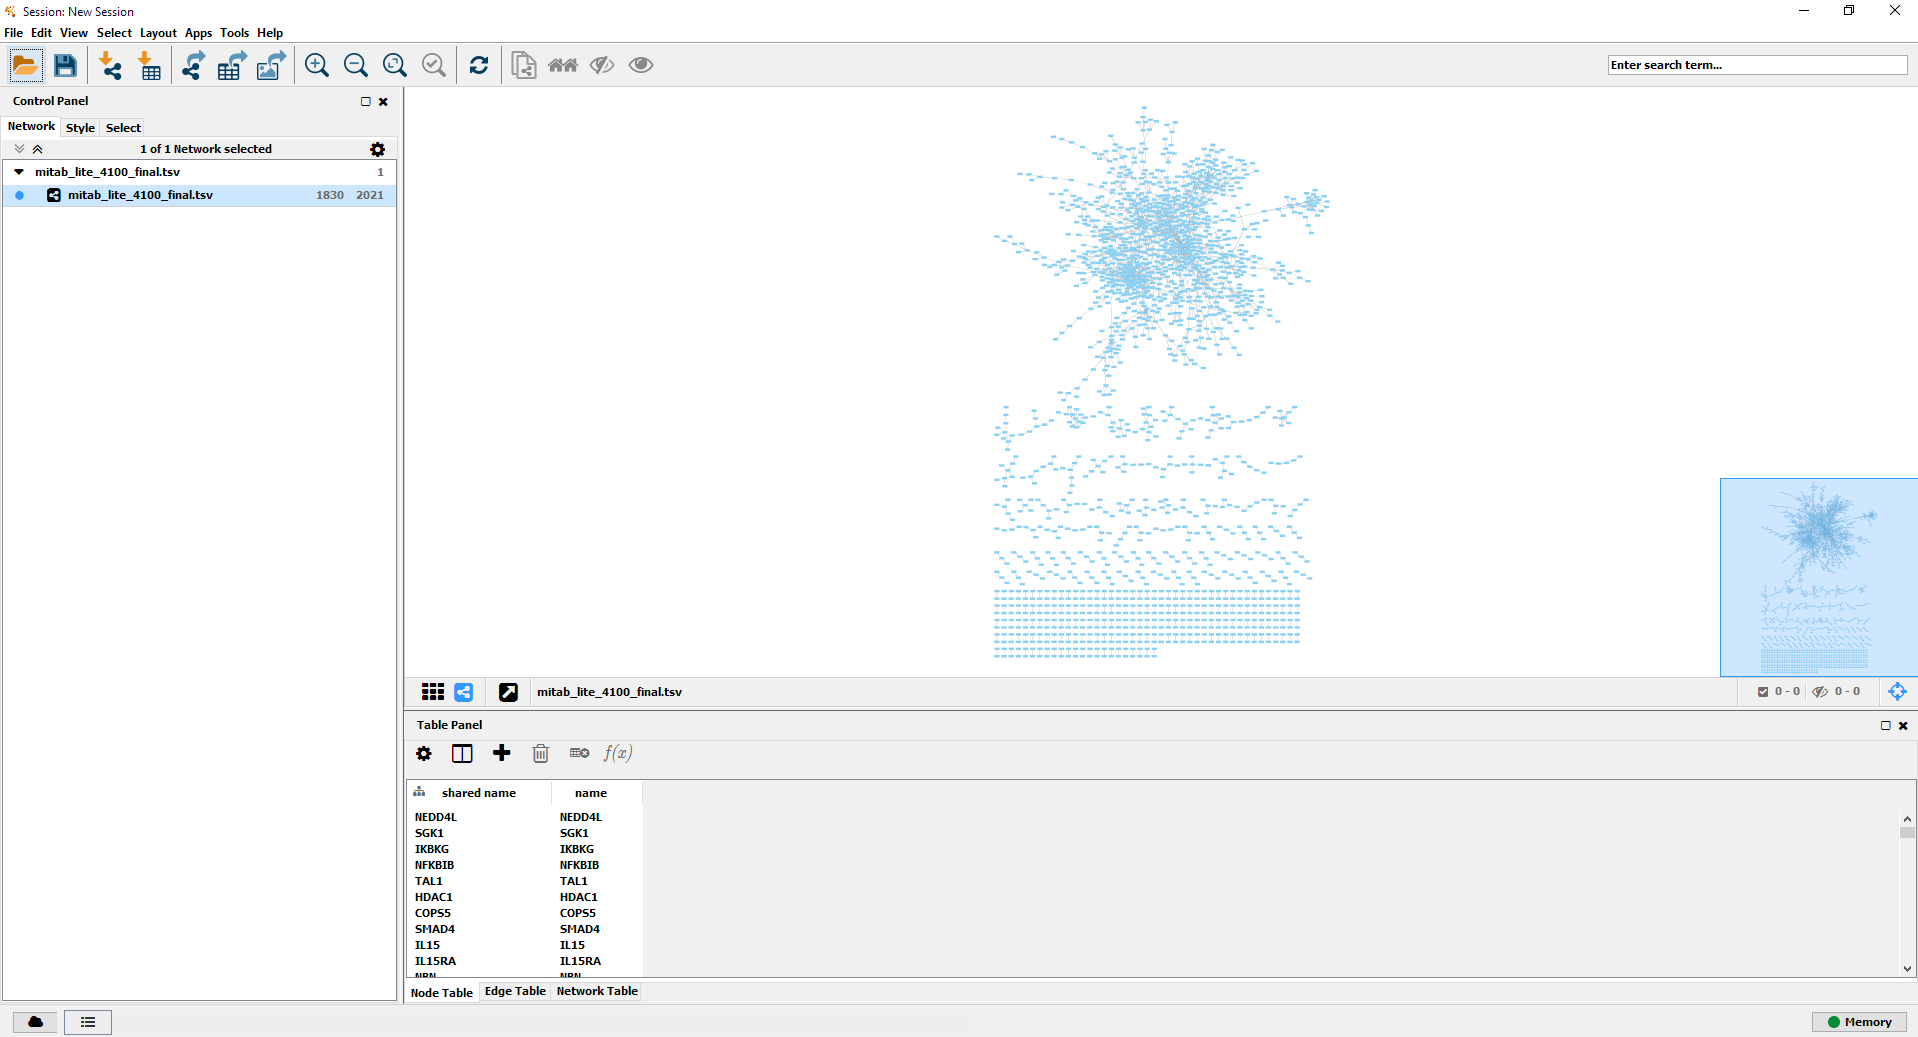
\includegraphics[width=15cm]{4-imported-network}
\end{figure}
\begin{figure}[h]
    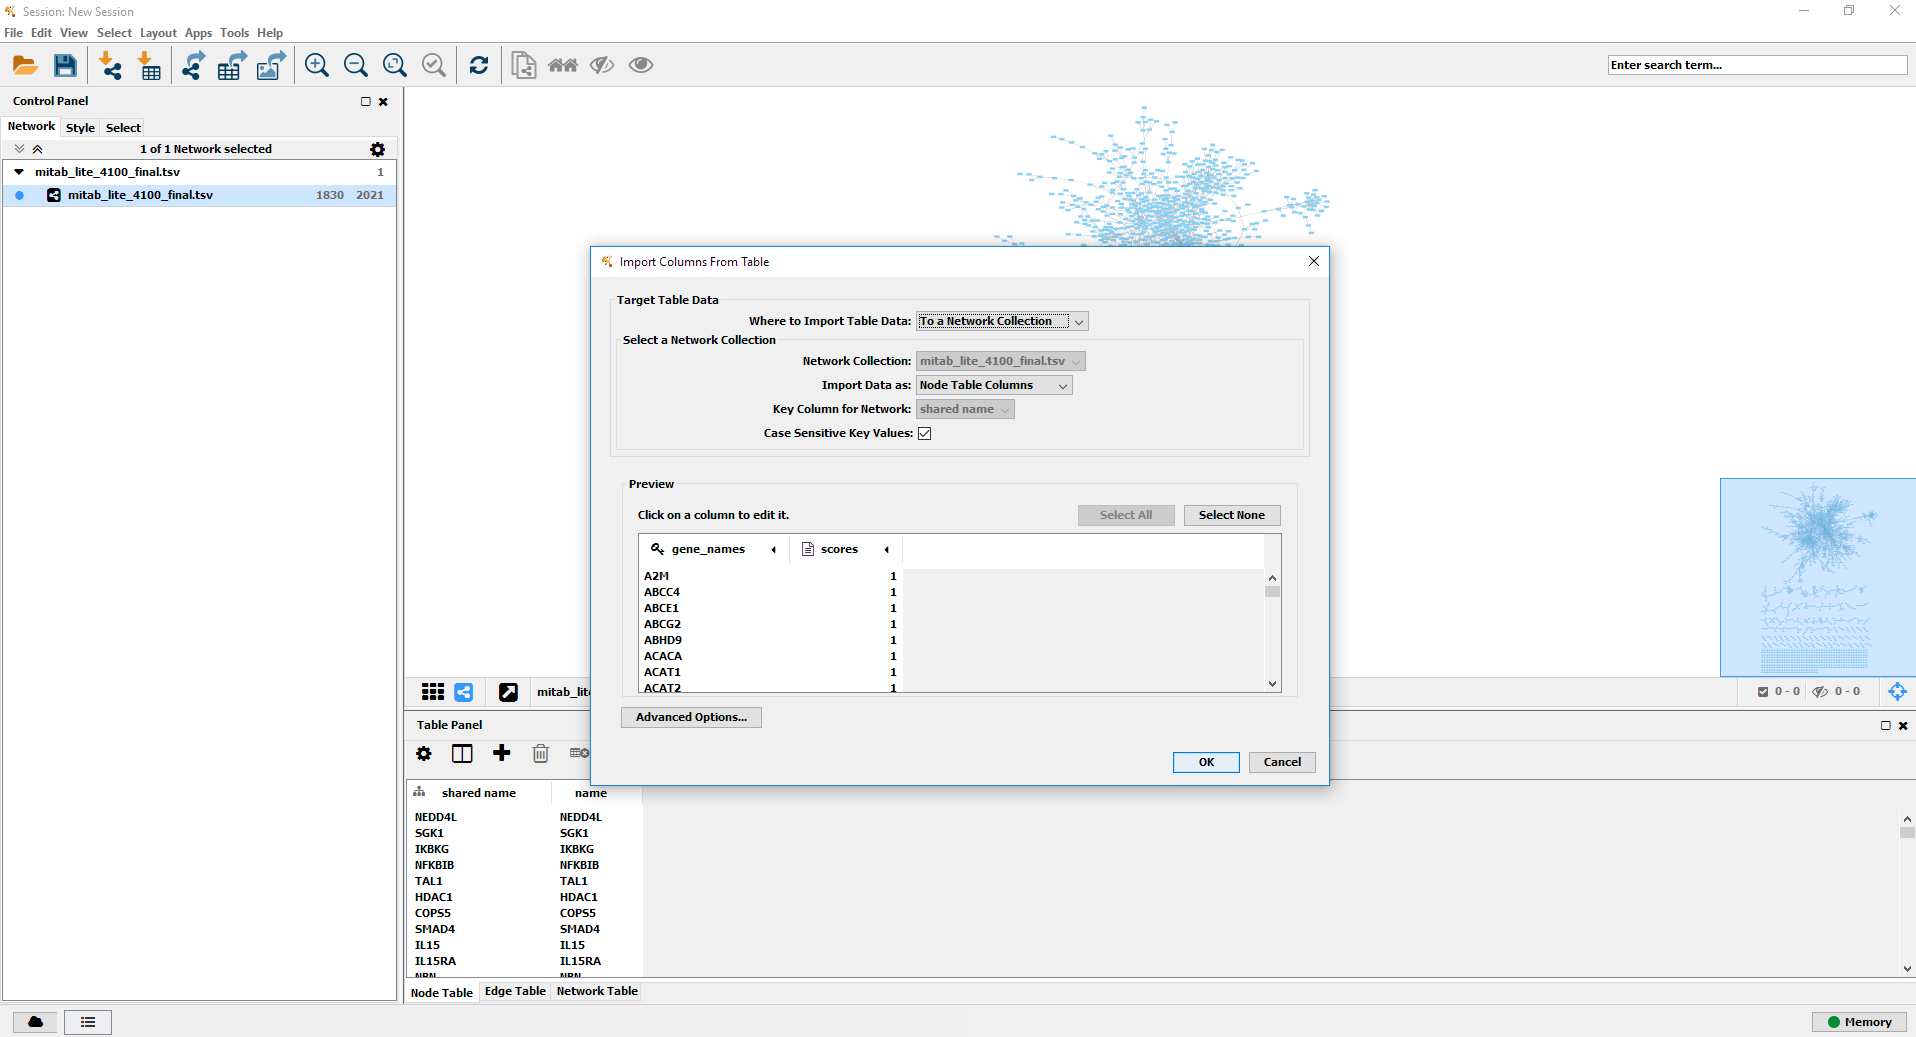
\includegraphics[width=15cm]{5-import-table}
\end{figure}
\begin{figure}[h]
    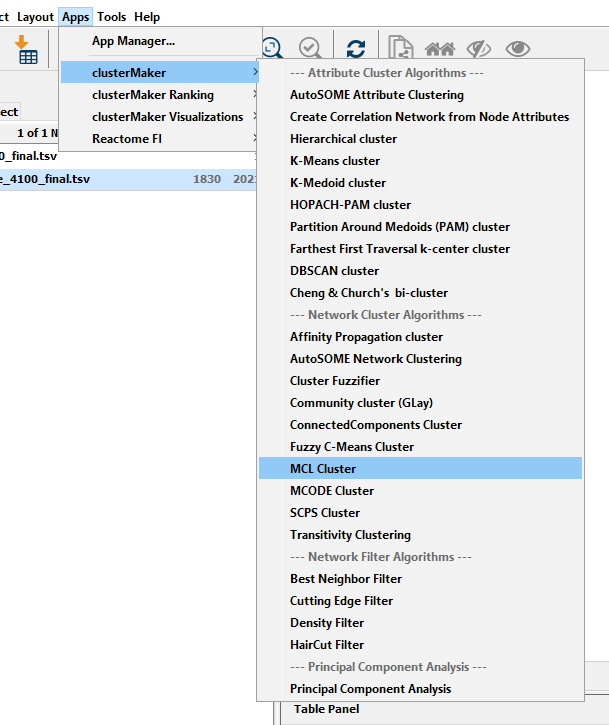
\includegraphics[width=15cm]{6-cluster}
\end{figure}
\begin{figure}[h]
    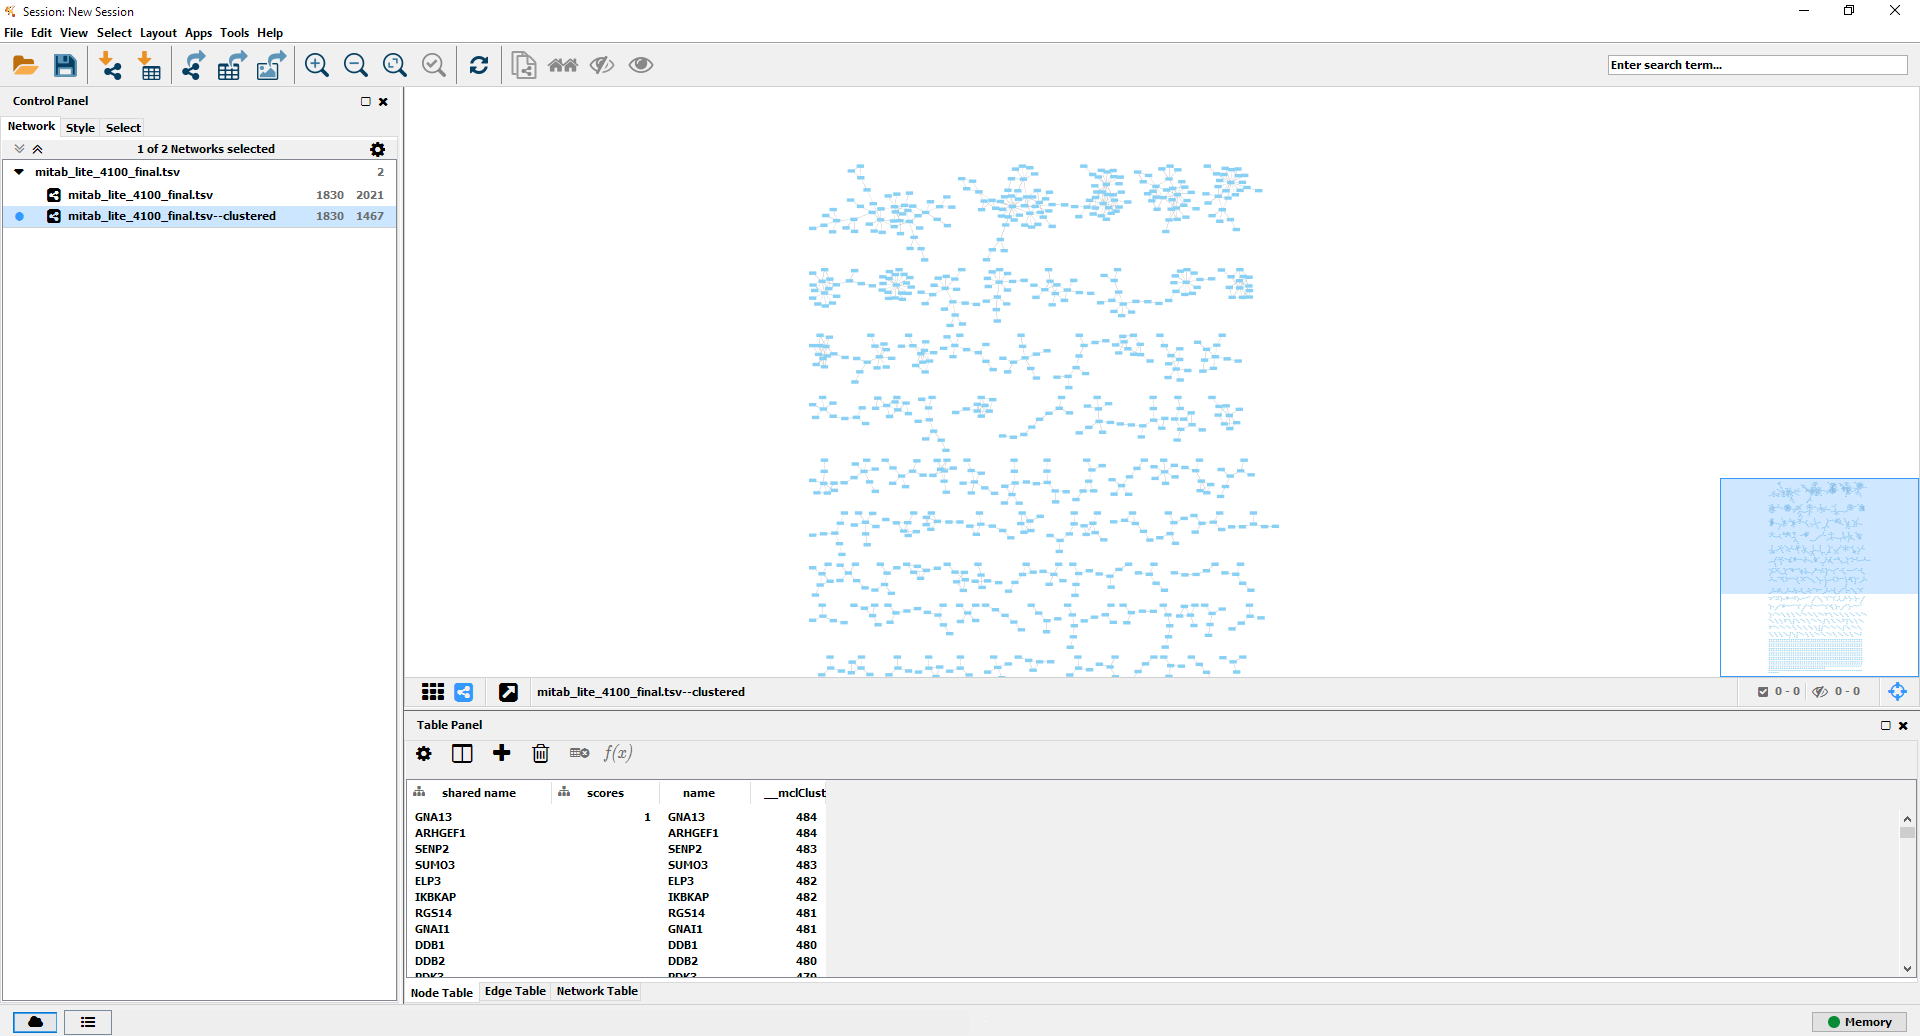
\includegraphics[width=15cm]{7-done-cluster}
\end{figure}
\begin{figure}[h]
    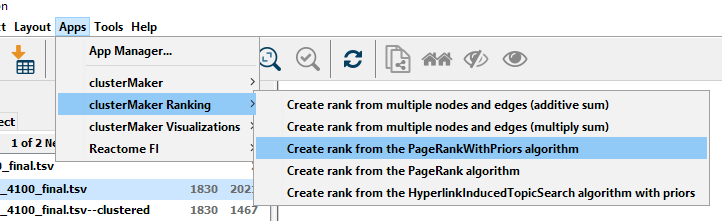
\includegraphics[width=15cm]{8-choose-ranking}
\end{figure}
\begin{figure}[h]
    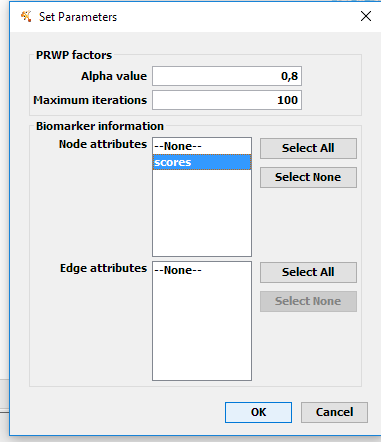
\includegraphics[width=15cm]{9-pagerank}
\end{figure}
\begin{figure}[h]
    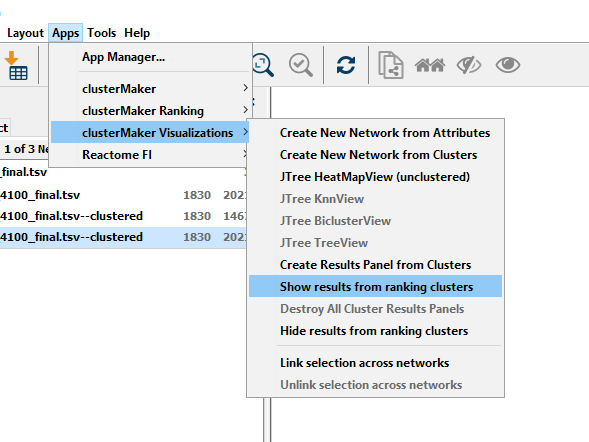
\includegraphics[width=15cm]{10-show-results}
\end{figure}
\begin{figure}[h]
    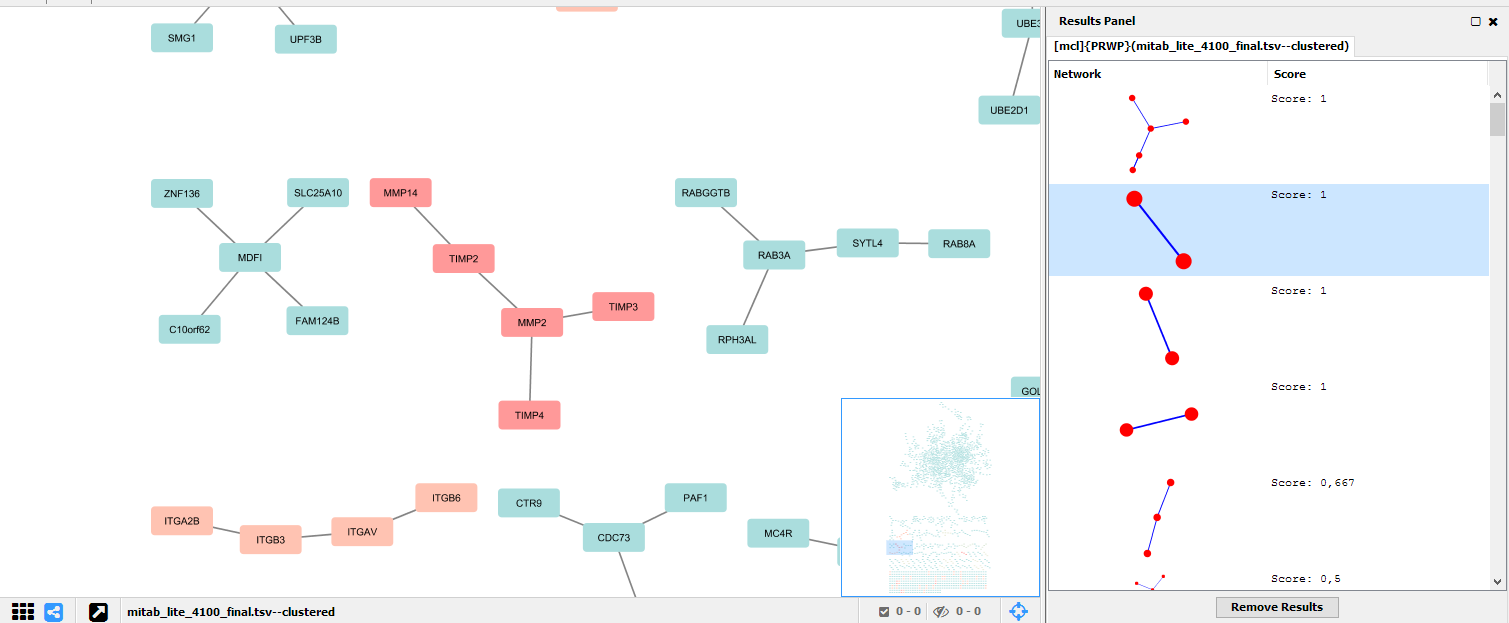
\includegraphics[width=15cm]{11-result-colors}
\end{figure}
\begin{figure}[h]
    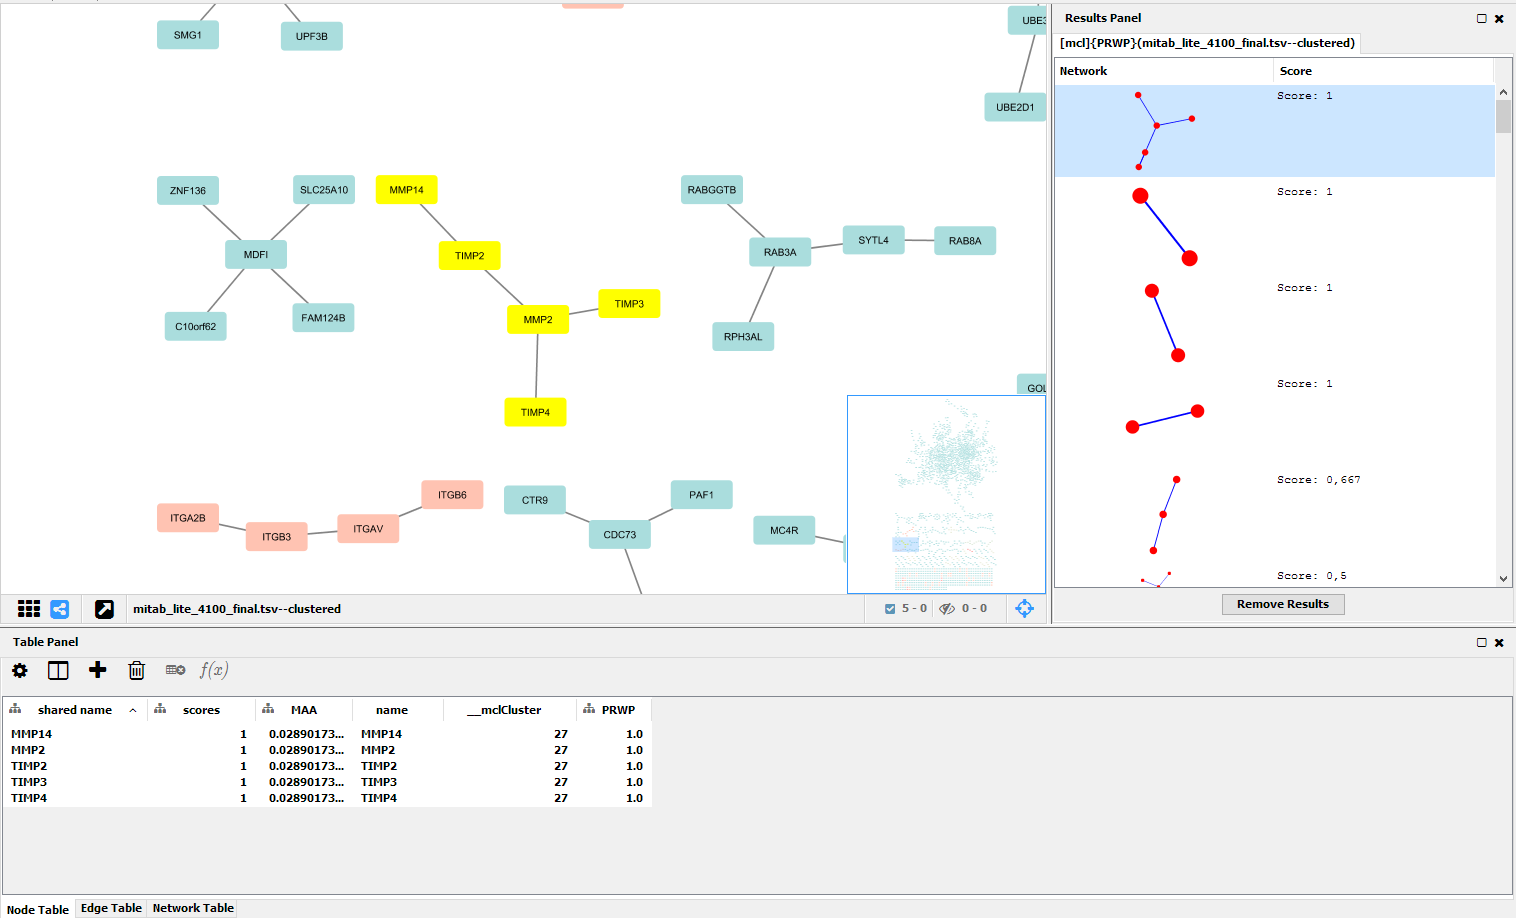
\includegraphics[width=15cm]{12-rank-selection}
\end{figure}

\chapter{Cytoscape}
\section{Intro}
The \textit{clusterMaker2} documentation for implementing new parts that is not
directly connected with clustering algorithms is non-existing. This part
explains the details about how it was done.

Cytoscape has a cookbook\cite{cytoscape-cookbook} listing a combination of best
practices and tips on how to start developing an app, add menues, panels,
algorithms, color schemes etc.. Instead of following all of these examples, we
have read through the existing code in clusterMaker2\cite{cm2-github} and tried
to structure the code of the contributions in Ranklust to match the structure
already implementet in clusterMaker2. Meaning that for each algorithm
implemented, they will all have a corresponding \textit{Factory} class and a
\textit{Context class}. For the panel that was implemented, it has a pure panel
class with Java Swing\cite{java-swing} settings, a panel task class, create
panel task class and destroy panel task class. % Make UML!

\section{Design}
\begin{figure}[H]
    \caption{Ranklust ranking algorithm relations}
    \label{fig:rank-alg}
    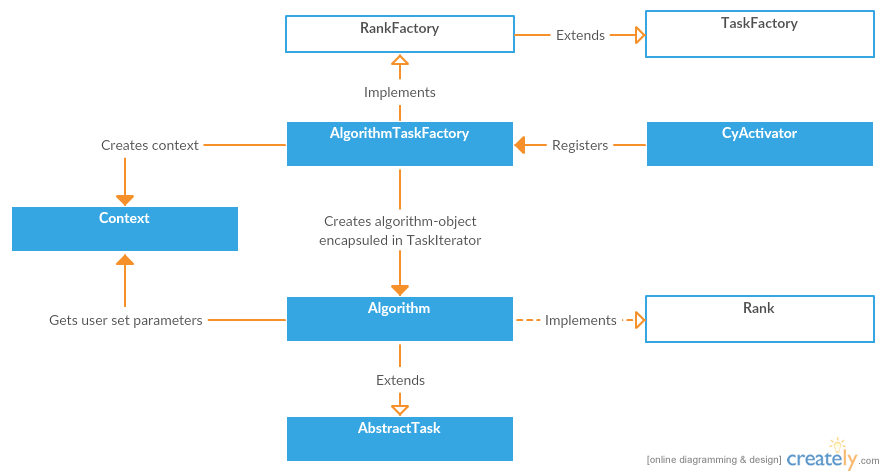
\includegraphics[width=\textwidth]{ranklust-algorithm}
\end{figure}
\begin{figure}[H]
    \caption{Ranklust ranking panel relations}
    \label{fig:rank-panel}
    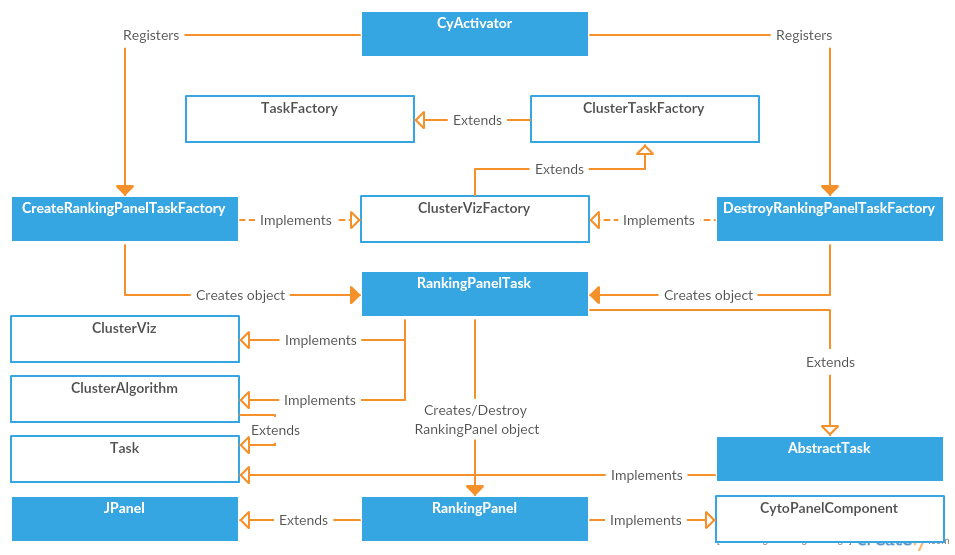
\includegraphics[width=\textwidth]{ranklust-panel}
\end{figure}

\section{Maven and the POM file}
The POM-file has to be updated because libraries connected to the pdf exporting
functionality is outdated. Updating the libraries, imports and the usage of
these libraries in the source code is enough to make the whole project compile.
Also, in order to get the third-party libraries to JUNG\cite{jung} into the
project, the three packages that is being used has to be added to the POM file
and the classes they contain has to be exposed in the OSGi
module\cite{osgi-felix}. Exposing the JUNG classes inside the clusterMaker2 OSGi
bundle could have been avoided if JUNG had OSGi modules in maven repositories,
but there is only 2 out of 3 OSGi ready modules that was needed in this project.
These were the changes needed:

Changed which packages was exported through the OSGi module.

\begin{lstlisting}[language=XML, caption={POM-file OSGi changes}]
<Export-Package>!${bundle.namespace}.*,*;-split-package:=merge-first</Export-Package>
\end{lstlisting}

Added these dependencies

\begin{lstlisting}[language=XML, caption={POM-file JUNG changes}]
<dependency>
    <groupId>net.sf.jung</groupId>
    <artifactId>jung-graph-impl</artifactId>
    <version>2.1</version>
</dependency>
<dependency>
    <groupId>net.sf.jung</groupId>
    <artifactId>jung-algorithms</artifactId>
    <version>2.1</version>
</dependency>
<dependency>
    <groupId>net.sf.jung</groupId>
    <artifactId>jung-api</artifactId>
    <version>2.1</version>
</dependency>
\end{lstlisting}

As seen here, the 3 modules needed is jung-api, jung-graph-impl and
jung-algorithms. Only the first 2 was OSGi ready. An alternative could have been
to create a OSGi ready module of the jung-algorithms module, but taking on the
responsibility for having a module updated at all times is too much for a single
person. However, it could become the clusterMaker2's developers responsbility to
create and update all 3 modules. The last alternative is to find other graph
ranking algorithm libraries like Apache Spark\cite{spark}, thas is OSGi ready.
The reason for not choosing Apache Spark is that it was not discovered until all
of the Java implementation was finished, making it a future goal to reach, at
best.

\section{App registration and java class connections}
First step of registration is to register a \textit{service listener} to the
already existing clusterMaker2 \textit{CyActivator}. Here we describe the name
of java methods in the \textit{clusterManager} class with strings. These two
methods for adding and removing ranking algorithms registers and unregisters the
algorithms to the \textit{App} menu in Cytoscape, making them accessible for the
user through the GUI. Registering a new service listener is a way of keeping the
Ranklust part out of clusterMaker2. Also, creating a standalone plugin at
a later stage will be easier if Ranklust is properly compartmentalized.

% insert code example (lstlistings)

The \textit{RankFactory} class is a java public interface used for each of the
ranking cluster algorithms, HITS, PR, PRWP, MAA and MAM. A class applying the
task factory design pattern is meant to deliver an object of the class it is
related to\cite{factory-design}, and it can return different types of a class
that has the same java superclass\cite{java-superclass}. In this case, each
class implementing the \textit{RankFactory} will only have a single class to
return. The RankFactory class also creates a \textit{Context} class, which binds
information the user can input to the GUI to variables, allowing the algorithm
to gain access to parameter information about the algorithms before they run.

\section{Algorithm}
% Rank interface
\section{GUI}
\subsection{Algorithm menus}
Much of these menus
\subsection{Ranking panel}
The code for the \textit{RankingPanel} is a copy from the existing
\textit{ResultsPanel} in clusterMaker2. The results panel has some extra
information that is removed in the ranking panel. The ranking panel only
displays which clustering and ranking algorithm that was used and the network it
is used on, together with the score of each cluster sorted descendingly, having
the highest ranked cluster at the top. The ranking panel will display in the
same place as the results panel, to the right of the network view.

The panel supports multiple selection of clusters through the \textit{Control}
key on the keyboard, much like its existing behaviour on Windows when selecting
multiple directories or files in the \textit{File Explorer}. Selecting the
clusters in the panel will also select them in the network view, enabling the
user to use other Cytoscape utilities on the nodes/clusters selected, for
example create a new network based on only the selected nodes. The color of the
selected nodes will also change in the network view, when the user selects a
cluster in the ranking panel, providing visual feedback to the user, in order to
make it easier for the user to see where the selected nodes/clusters resides in
the network.

When tasking clusterMaker2 with showing the ranking panel, the color of the
nodes will also change. This is to visualize the rank of each cluster in the
network view to the user. Coloring the highest scoring clusters with red or
green and the lowest scoring with the opposite was the first and easiest
solution. There was made a choice to color the whole cluster according to the
rank it received, instead of individually color nodes according the their
contribution to the clusters rank. The user might be interested in choosing what
suits them best when it comes to this, so it might be implemented a menu for the
ranking panel in the future to best meet the users needs.

Taking color blind people into consideration red and green is not the
best combination. Colors resembling red and green in the form of hot-to-cold
colors that all types of colorblind people can view was therefore a criteria to
be met. A style satisfying these criteria will follow, having the hex value of
te color\cite{color-blindness3}, followed by the RGB value that was calculated
using a site that converts from hex to RGB values\cite{color-blindness2}.
\textit{\#ADD rgb\(170,221,221\)} for a blueish and cold color representing low
score. \textit{\#FEC rgb\(255,248,204\)} represents off-brown color that is a step
warmer than the blueish. The warmest color representing the highest scored
clusters is \textit{\#F99 rgb\(255,153,153\)}. The drawback with this color
combination is with people that has color blindness to the degree where they see
only greyscales. The colors low to high will go from grey to light grey to dark
gray, which does not seem logical. The color style might change if users
experience trouble having these colors representing the cluster ranks. 

\section{State of today}
The pull request\cite{git-pull-request} made from the Ranklust
contribution of this thesis has been accepted\cite{ranklust-accepted}, adding
3750 lines of code and deleting 1051. The changes was distributed across 50
files. The type of files edited ranges from the Maven POM-settings file and
.gitignore to plain Java source code files. Further changes will be made, as the
work on the Ranklust contribution will not end when this thesis is delivered.
One of the most recent changes to the contribution is that the
\textit{PageRankWithPriors} algorithm used to analyze the networks in this
thesis assumes undirected edges because of the
\textit{UndirectedSparseMultigraph} graph used, while for normal use, directed
edges is believed by us to be the most sought after choice. Therefore, the pull
request was hardcoded with directed edges. Choosing between directed and
undirected edges should be up to the users of clusterMaker2 and is on the
TODO-list of futures to implement.

\section{Known bugs}
\subsection{Menu bugs}
\paragraph{Unintentional execution of clustering algorithm}
\begin{enumerate}
    \item Open the clusterMaker2 clustering algorithm menu
    \item Select a clustering algorithm
    \item Exit the menu for the algorithm without running it
    \item Repeat step 1-2 and it results in running the previous algorithm that
        was exited
\end{enumerate}
This was the behaviour before Ranklust contributions was added to clusterMaker2,
so it might be clusterMaker2 or it might be Cytoscape itself. Most likely, the
way clusterMaker2 algorithms is started through its \textit{TaskFactory}'s needs
to be changed, but this is just a hunch and not based on any analysis.

\subsection{Ranking panel bugs}
It is a known bug with the style for node coloring that the ranking panel
causes. The colors in the nodes might flicker when several ranking algorithms
has been run and the colors of each node has changed several times. This is
probably related to the previous color style for the nodes and it will be fixed
in the future.

\chapter{Clustering} %% TODO: redundant
The clustering algorithms used to produce the clusters to rank will be AP and
MCL.

The clustered network can be constructed with AP, a clustering algorithm
\cite{affinity-propagation}. AP clustering concentrates on the nodes in the
network that are binding the rest of them together. Using affinity propagation
for clustering will produce results that represent a grouping of nodes that are
coupled by seemingly unimportant nodes to most clustering algorithms. But the AP
algorithm is good at expressing nodes that are not highly connected to many
nodes, but rather the nodes that are binding other highly connected nodes
together. This results in bigger clusters that can be a target for methods that
cure cancer by severing the interaction between biomarker genes.

It is also discussed how AP performs versus Markov clustering \cite{ap-vs-mcl}.
And since Markov algorithm performs better on protein interaction, it will also
be used to cluster the networks. An analysis between the rankings that come from
the Markov and AP clusterings will be performed, which hopefully will give
concrete results as to the pro's and con's of each algorithm. Some questions
should be raised as the analysis is done. For example, is both of the algorithms
good, but have different uses, even if they are not directly involved with the
ranking done after the clustering?  Are either AP or Markov useless for
a particular type of ranking afterwards?

The information provided through the whole process from what type of nodes
(protein or gene), interaction between the nodes and what kind of biomarker we
want to identify are all factors that will have a great impact on how all of
this should be combined. The order of operations on the network will also effect
the result. For example, AP clustering may create a few big clusters and many
small ones. At this stage, the results will consist of the biggest clusters
constructed from AP clustering that has focus on pure connection between nodes
and not their attributes. At this point, the cluster ranking algorithm of
Ranklust will be run in order to produce a picture of potential biomarkers. This
picture is the first and simplest step that will be used as a result for an
analysis. The analysis in this thesis will focus on validating the cluster
ranking scores as ways of indicating potential biomarkers. 

\section{Clustering} %% TODO: redundant
To cluster or not to cluster is the question here. PPI networks already have
a great deal of edges and can be seen as clusters that we should not alter. On
the other hand, using clustering algorithms to make clusters out of
PPI-networks gives us the more control over the clusters and has the potential
to identify protein complexes\cite{ap-vs-mcl}. How big they should be, how many
of them we want, should we cluster on a certain attribute, or even several? We
have chosen to go with the \textit{Markov Cluster}(MCL)\cite{mcl} clustering
algorithm in \textit{clusterMaker2}, without any limitations to the amount of
clusters. We prototyped Ranklust with \textit{Affinity
Propagation}(AP)\cite{affinity-propagation} because of its ease of use and low
execution time, but it has been proven through a comparison between MCL and AP,
that concluded with MCL having better performance in many aspects when it came
to cluster unweighted (binary interactions) PPI networks\cite{ap-vs-mcl}. These
aspects being noise tolerance and more robust behaviour.

\section{Ranking clusters}
We have used five algorithms to rank the clusters, MAA, MAM, PR, PRWR and HITS.
The first two are simple algorithms that through addition or multiplication
calculates a cluster average score. The three others utilize network ranking
algorithms from the Java JUNG\cite{jung} library.

Every algorithm implemented in Ranklust for ranking clusters except HITS takes
node and/or edge scores as input for calculating the scores for each cluster.

\subsection{Multiple Attribute Additive Method (MAA)}
Multiple attribute additive method is the first algorithm implemented.  The user
has the option of choosing an unlimited amount of attributes from nodes and
edges.

It goes through all of the nodes in each cluster and sums up the number-
attributes the user chose. Each cluster is then ranked based on the average sum
in each cluster and ranked descending, with the highest ranking cluster as the
most likely prostate cancer biomarker cluster.

There is a question as to how to rank the edges in the cluster. We chose to rank
each edge as it is listed to the user in Cytoscape. So if it is listed only once
time in the edge table, it will only be scored additively once. This decision
was based on simplicity. To not represent the edge as something the user did not
define it as, or is unable to understand. Some clustering algorithms might
assign the same node or edge to several clusters, though this is not the case
with the algorithms we use in this thesis. Support for this is only implemented
by MAA and MAM, as they were implemented before a final decision on which
clustering algorithms should be used. If MAA/MAM discovers this special case of
several scores for a single node or edge, it will assign it the highest value.
The reason for leaving this feature in Ranklust is to have an example on how it
can be done, should it be a problem in the future.

\subsection{Multiple Attribute Multiplication Method (MAM)}
Multiple attribute multiplication method is to some degree redundant,
considering what exists from before in Ranklust. The only difference from MAA is
the scale the scores will be in. MAA adds the scores from each node and edge in
the cluster through addition, MAM does it with multiplication.

A problem that occurs with multiplication is calculating scores for clusters
that contain nodes with a score between 0 and 1, since the score would decrease
to such a degree that it would be difficult to work with when normalizing the
scores. The solution we have chosen for this is to make a new score from the
old score, and add 1.0 to it. This way, when the existing average score in the
cluster is multiplied with the new score, it will always increase, unless the
old value was 0.0, then it will stay the same. In the case of values above 1,
they will also be given an increase by 1.0 in order to keep it consistent if the
scores vary between 0 to \textit{n}. % TODO: discussion -> could be normalized

\subsection{PageRank (PR) and Personalized PageRank (PRWP)}
A Random Walks\cite{random-walks2} algorithm which used priors, called
seed-weighted random walks ranking \cite{sw-rwr}, proved to be effective at
prioritizing biomarker candidates. PageRank (PR) is an algorithm based on the
Random Walks principle, and it is contained inside the Java library
\textit{JUNG}\cite{jung}.  PR was previously used by Google to rank webpages
\cite{pagerank}.  Personalized PageRank (PRWP)\cite{pr-bio} is a modified
version of PR, where nodes and edges can be assigned a score prior to the PR's
traversal of the network. PR can have values assigned to the edges, but it does
not require any scores in order to rank clusters, which PRWP does. Personalized
PageRank is abbreviated PRWP because of the Java classname it has in the Java
JUNG library
- \textit{PageRankWithPriors}.

The difference between MAA and MAM compared to PR and PRWP is how the network is
scored. MAA and MAM calculates the score for each cluster by summing up the
attributes in edges and nodes according to the cluster attribute. PRWP scores
the current network regardless of the clustering attribute. 

MCL gives the option of creating a clustered network, which opens up the
possibility of working with two types of the same network, non-clustered and
clustered. They both have the clustering attribute in the network, edge and node
table, so that the ranking algorithms are able to score the clusters.  PRWP
scores the currently selected network in Cytoscape, resulting in the option of
scoring the non-clustered network or clustered network. The last option gives
the clustering algorithm a bigger impact on the score, because the clustered
network has perturbated edges between nodes that is not in the same cluster. MCL
in Cytoscape can show the "inter-cluster" connecting edges, which is the egdes
that was perturbed during clustering. This last option is a combination of the
two others. It will be visually close to the clustered network, but algorithms
that run on the network with inter-cluster edges will have the same result as
the network only containing the cluster attribute.

Implementation wise, there is also a difference in how the scores are stored in
the network after the algorithm is finished executing. All the scores are stored
in the nodes. To give information to the user about the scores the edges
received, each edge will display the total score for the cluster it is a member
of, just like the nodes.

\subsection{Hyperlink-Induced Topic Search}
Hyperlink-Induced Topic Search, HITS, an algorithm that is similar to PageRank,
was developed around the same time \cite{hits}\cite{hits-origin} and is also
contained within the Java JUNG library. HITS will not be used to calculate
cluster scores and ranks, due to the fact that it does not require any form of
weighting in nodes or edges. Though, it can be used in combination with other
ranking algorithms through the use of MAM or MAA. 

An example of this could be running PRWP with a score attribute, then HITS on
the same network. The next step would be to combine the two scores from PRWP and
HITS with MAA. Though, the idea of achieving novel information on network
biomarkers for prostate cancer through this workflow is pure speculation, and we
have chosen to use each ranking algorithm separately, in order to limit the
amount of datasets to analyze.

\subsection{PR, PRWP and HITS}
Because PR, PRWP and HITS rely on an alpha variable controlling the probability
of a reset in the traversal of the network. This "traversal reset" is
automatically triggered if the algorithm hits a node with no outgoing edges. As
the clustering algorithms might change the edges in the network, the outcome of
performing ranking on a cluster-created network, or a network with only
a cluster attribute to identify the clusters, can be potentially vastly
different. The alpha value parameter will be set to 0.775. This is because the
results from running the similar algorithm "seed-weighted random walks ranking"
was achieved with an alpha value of 0.7 \cite{sw-rwr}. There is a report of
Google having used a value of 0.85 \cite{pr-parameters} as the alpha value, so
the average of these two should provide for a alpha value to start with.

Another parameter for PR, PRWP and HITS is the iteration parameter. For each
iteration of these algorithms, they assign a value to each node. Performing
multiple iterations contribute to stabilize these values. In the previously
mentioned report from Google \cite{pr-parameters}, a \textit{n x n} matrix where
\textit{n} was about 25 billion, required about 50 - 100 iterations in order to
stabilize the node values. Iterations needed to stabilize increase with the size
of the network, therefore the iteration value to start with will be 100, should
it not take too long to calculate. It should be way more than needed, because
the size of the network used to test with contains about 1500 nodes and 1500
edges.


\chapter{Programming specifics}
\section{Tables vs pure OO}
One thing in particular that deserves to be mentioned is the way networks are
handled. The \textit{CyNode} objects themselves does not contain much. This is
because all of the information is saved in the form of plain cells in a
spreadsheet. This may at first seem like a way to make it easy to show
information to the user, but it is also a way of working more efficient with
network data (insert: reference to working with tables on networks is
efficient). Creating objects with attributes for each node in a huge network
will increase the amount of overhead by a pretty noticeable amount. Working with
all of the information in the way of a spreadsheet with rows and columns
includes a decrease in overhead. A new node is a new row in the node table, so
in relation to building the network structure, it is not a complex abstraction.
The difference comes in when the nodes have several attributes. 

In a table or spreadsheet, attributes can be represented as a single column and
be created once for the whole network, instead of once for each node object
created. This assumes that getting the objects out of the table is possible by
either indexing on a number for arrays, or a unique key for map structures.
The result is both a lookup, insertion and deletion time of O(1). These times is
as low as the Big-O notation goes in terms of speed related to the size of
a collection inside a data structure. So both the creation of objects goes
down, and the retrieval of attribute information is as low as it is possible to
get, when we choose to represent the time by Big-O notation. The only drawback
with this implementation is that there is no current type of wrapper around the
row and column system. So the retrieval of information is not done the most
intuitive way. But this is the way Cytoscape works as a whole, so changing the
way this works can either be done through changing the Cytoscape source code, or
implementing a wrapper as a standalone function inside clusterMaker2 or as
a standalone plugin. In Ranklust, an extension to the existing
\textit{NodeCluster} class was used to keep scoring information about nodes in
clusters.

\section{Changes in existing classes}
\subsection{NodeCluster}
\begin{verbatim}
/**
 * In it's simplist form, a Cluster is a group of nodes that represents the
 * nodes that are grouped together as the result of a clustering algorithm
 * of some sort.  A more complicated form of a cluster could include clusters
 * as part of the list, which complicates this class a little....
 */
\end{verbatim}

This comment is in the NodeCluster class. In the Ranklust implementation,
several attributes and methods has been added to this class. Saving the
temporary state of the scores to the clusters could have been done in the node
and edge-tables in Cytoscape, but it was faster both implementation- and
performance-wise to extend the NodeCluster class. Also, a criteria for extending
this class was that the existing API of this class should not change, in order
to avoid unneccessary changes for other classes in clusterMaker2, that is not
a part of the Ranklust contribution. 

Additions to NodeCluster contains variables representing cluster \textit{score},
\textit{rank} and a \textit{HashMap} from a cluster-node's SUID to its score.
The map and rank variables is part of a previous implementation and can be
removed. Adding node scores to the cluster and normalizing it afterwards.

\textbf{Common responsibilities introduced in Ranklust}

\begin{itemize}
    \item Adding node scores to the cluster (ranking algorithm related)
    \item Normalizing cluster scores for a list of clusters (static method)
    \item Calculating min/max/avg scores for a list of clusters (static method)
    \item Ranking a list of clusters by their score and set their rank
        accordingly (ranking panel related)
\end{itemize}

\subsection{GraphicsExportPanel}
Minor changes were done to GraphicsExportPanel when a new class for handling PDF
documents was introduced. This was the result from the need to change the maven
dependency to use the "com.itext"\cite{itext} repository location instead of
a location from "com.lowagie" because the library was relocated
\cite{lowagie-to-itext}.

\section{New classes}
\subsection{ClusterUtils}
\textit{ClusterUtils} is a new class implemented in the Ranklust contribution.
It is used by every cluster ranking algorithm implemented in Ranklust. To some
degree it has a common responsibility with the \textit{ModelUtils} class from
clusterMaker2. The difference being that ClusterUtils is focused on inserting
scores in tables related to cluster ranks. It also normalizes scores not
directly related to a NodeCluster, but rather a group of \textit{CyNodes}, that
has mapped their SUID in Cytoscape to a score received from a ranking algorithm.

\textbf{Common responsibilities introduced in Ranklust}

\begin{itemize}
    \item Getting cluster attribute based on CyNetwork
    \item Getting ranking attribute based on CyNetwork
    \item Ranking clusters firstly by score, secondly by cluster number
        (assuming a small cluster number is a bigger cluster)
    \item Fetching ranking results based on CyNetwork (ranking panel utility)
    \item Fetching clusters based on CyNetwork (ranking algorithm utility)
    \item Add score to a NodeCluster based on specified attribute column and
        CyRow to get it from
    \item Insert cluster scores into the default node- and edge-tables
    \item A simplified way of creating columns based on a specific column name,
        attribute class, table to create column in and immutability status
\end{itemize}

\section{Handling nodes and edges}
Recipe for working the nodes and edges: The steps are almost equal for
calculating both node and edge scores. How the edges are handled depends on what
direction they have. Are they undirected, directed, or unidirected. In the
current version of Ranklust, \textit{PageRankWithPriors} assumes undirected,
\textit{PageRank} and \textit{HITS} assumes directed. \textit{MAA} adds the
score from the edge to the cluster and \textit{MAM} multiplies the highest score
found as an edge attribute with the current cluster score. MAM and MAA assumes
the score is directed corresponding with source and target nodes in the edge
table of Cytoscape.

\begin{enumerate}
    \item Add score to the cluster
    \item Repeat step 1-2 for every edge
    \item Sort clusters based on rank and create a column to represent the
        cluster score
    \item Create single node score from cluster
\end{enumerate}

\chapter{Interpreting Ranklust results}
This was done solely by Python scripting, from formatting the data retrieved
from databases in order to construct networks in Cytoscape, to cleaning the
results exported from Ranklust, and analyzing the cleaned data.

\section{Network creation}
The network was created with protein interaction data from iRefWeb
\cite{irefweb}. 

\begin{figure}[H]
    \centering
    \caption{iRefWeb network query}
    \label{fig:irefweb}
    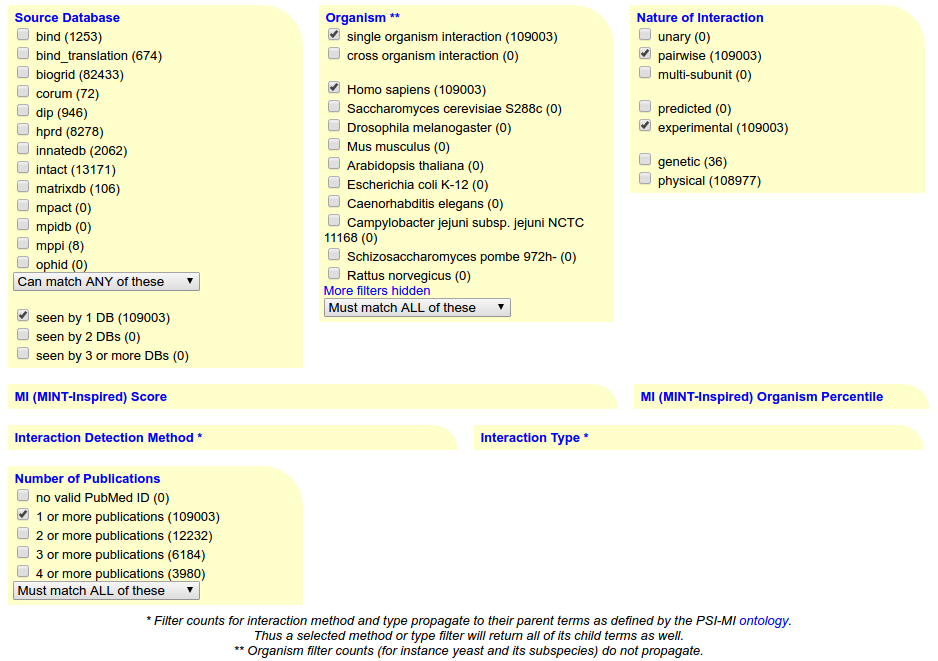
\includegraphics[width=15cm]{mitab_lite_109276}
\end{figure}

% change this from MITAB to MITAB-MINI!!!
It was downloaded in the MITAB format 

